\documentclass[a4paper,11pt]{article}
\usepackage{graphicx}
\usepackage{breqn}
\usepackage{pmisubmit}

\begin{document}

\initpmisubmision{2} % assignment number
{Shashank Shailabh}   % your name
{170655}	% your roll number

\begin{pmisolution}
%A vector symbol $\vb$, a symbol in blackboard font $\bR$, a symbol in calligraphic font $\cA$, \red{some} \green{colored} \blue{text}
\begin{enumerate}
    \item The equation 4 defines the expected complete data log posterior as
\[\bE_{\cY_{p}}[\log p(\boldsymbol\theta|\cD_{0} \cup (\cX_{p},\cY_{p}))]\]
The batch \({\cD}'\) is find such that it covers whole data variation which can be \(\cD_{0} \cup \cD_{p}\). The unavailability of complete data is removed using posterior expectation as.
\begin{align*}
    \bE_{\cY_{p}}[\log p(\boldsymbol\theta|\cD_{0} \cup {\cD}')] &\approx \bE_{\cY_{p}}[\log p(\boldsymbol\theta|\cD_{0} \cup \cD_{p})]\\
    &\approx \log p(\boldsymbol\theta|\cD_{0}) + \sum_{m=1}^{M}\cL_{m}\\
\end{align*}
The sparse approximation is selecting \(B\) points from \(M\) points and with objective function  to minimize \(|| \sum_{m=1}^{M}\cL_{m} - \sum_{m=1}^{M}w_{m}\cL_{m}||^{2}\)  subject to \(w_{m}\in \{0,1\}\) and \(\sum_{m=1}^{M}w_{m} \leq B\). The idea above is true as sparse approximation where B points approximates the updated expected data log posterior to expected complete data log posterior.
\item The relaxed objective is
\[\min_{w} (1-\vw)^T\vK(1-\vw)\] such that \(w_{m}\) is non-negative and \(\sum_{m=1}^{M}w_{m}||\cL_{m}|| = \sum_{m=1}^{M}||\cL_{m}||\).\\
The original objective function constraint is NP-hard so the relaxed objective uses trick of constrain optimization. The original constrain is changed to non-negative constrain where greedily B points are chosen in one by one fashion followed by projecting to the original constrain space. The selection is performed such that the point chosen takes closest to the complete posterior.
\item The acquisition function proposed in the paper gave closed form solution for linear supervised model. The non-linear supervised learning models can use random feature projection using MC approximation since acquisition function won't be available. The Equation(16) in the paper describes the approximate projection.
\[ \hat{\cL_{n}} = \frac{1}{\sqrt{J}} [\cL_{n}(\boldsymbol\theta_1), ..., \cL_{n}(\boldsymbol\theta_{J})]^T\]
where \(\boldsymbol\theta_j \sim \hat{\pi}\) and \(\hat{\cL_{n}}\)  is J-dimensional projection of \(\cL_{n}\).
\end{enumerate}
\end{pmisolution}

\begin{pmisolution} 
Given the input \hspace{1em} \(x_{1}, x_{2},..,x_{N} \sim \mathcal{N}(x,|\mu,\beta^{-1})\) and prior on \(\mu \sim \mathcal{N}(\mu|\mu_{0},s_{0})\) and \(\beta \sim Gamma(\beta|a,b)\).\\\\
\textbf{Conditional Posterior}\\
Using Bayes rule for conditional posterior calculation.\\
\[p(\mu|x,\beta^{-1}) = \frac{p(x|\mu,\beta^{-1}) p(\mu|\mu_{0},s_{0})}{\int p(x|\mu,\beta^{-1})p(\mu)d\mu}\]
Both likelihood and prior are gaussian, using squares trick and assume mean = \(\mu_{N}\), variance = \( \sigma_{N}^{2}\) and \(\bar{x} = \frac{1}{N}\sum_{i=1}^{N}x_{i}\) where 
\[\mu_{N} = \frac{\mu\beta^{-1}}{Ns_{0}+\beta^{-1}} + \frac{Ns_{0}\bar{x}}{Ns_{0}+\beta^{-1}}\]
\[\frac{1}{\sigma_{N}^{2}} = \frac{1}{s_{0}} + N\beta\]
Now again using Bayes rule for \(\beta\) posterior calculation.\\
\[p(\beta|x,\mu) = \frac{p(x|\mu,\beta^{-1}) p(\beta|a,b)}{\int p(x|\mu,\beta^{-1})p(\beta)d\beta}\]
Now the conditional on \(\beta\) is defined by \(Gamma(\beta | a_{N},b_{N})\) where \\
\[a_{N} = a + \frac{N}{2}\] and \[ b_{N} = b + \frac{\sum_{i=1}^{N} (x_{i} - \mu)^{2}}{2}\]\\

\textbf{Gibbs Sampling}\\
The random samples are iteratively drawn from the conditional posteriors. When the sampling is long run enough (convergence achieved), then the samples are from the joint posterior. These are the steps for Gibbs sampler -
\begin{itemize}
    \item Initialize \(\mu^{(0)}\)
    \item For \(s = 1, 2,..., S\)
    \begin{itemize}
        \item Draw a random sample for \(\beta\) as \(\beta^{(s)} \sim p(\beta |x,\mu^{(s-1)})\)
        \item Draw a random sample for \(\mu\) as \(\mu^{(s)} \sim p(\mu |x,\beta^{(s)})\)
    \end{itemize}
\end{itemize}
These pairs of samples \((\mu^{s},\beta^{s})^{S}_{s=1}\) represent joint posterior of \(\mu\) and \(\beta\).
\end{pmisolution}

\begin{pmisolution}
\begin{enumerate}
    \item The above prior on \(\vw\) penalises differently for each weight and forces the weights towards zero. Intuitively, the prior is classifying the features in two groups.
    \item The conditional posterior on \(\vw\) is calculated as     \(p(\vy|\vw,\vX, \sigma^2) = \mathcal{N}(\vy|\vX\vw,\sigma^2\vI)\) and \(p(\vw|\sigma^2, \gamma) = \mathcal{N}(\vw|\sigma^2\vK)\) where \(\vK\) is \(D\times 1 \) diagonal matrix withe \(\vK = diag(\kappa_{\gamma 1},..,\kappa_{\gamma D})\) 
    \[ p(\vw|\vy,\vX,\sigma^2, \gamma) \propto p(\vy|\vw,\vX, \sigma^2)p(\vw|\sigma^2, \gamma)\]
    Now, \(p(\vw|\vy,\vX,\sigma^2, \gamma) = \mathcal{N}(\vw|\boldsymbol\mu_N,\vSigma_N)\) where \(\vSigma_N = \sigma^2(\vX^T\vX + \vK^{-1})^{-1}\) and \(\boldsymbol\mu_N = (\vX^T\vX + \vK^{-1})^{-1}\vX^T\vy\).\\\\
    The EM algorithm -\\
    \textbf{Expectation Step}:
    \begin{align*}
        \log p(\vw,\vy | \vX,\sigma^2, \gamma) &= \log(p(\vy|\vw,\vX, \sigma^2)) + \log(p(\vw|\sigma^2, \gamma))\\
         &= \frac{-1}{2\sigma^2}(\vy - \vX\vw)^T(\vy - \vX\vw) - \frac{(D+N)\log(2\pi\sigma^2)}{2} \\
         & \hspace{7em}- \frac{\vw^T\vK\vw}{2\sigma^2} - \frac{1}{2}\sum_{d=1}^{D}\log (\kappa_{\gamma d})\\
         &= \frac{-1}{2\sigma^2}(\vy^T\vy - 2\vy^T\vX\vw + \vw^T\vX^T\vX + \vw^T\vK^{-1}\vw)
         - \frac{(D+N)\log(2\pi\sigma^2)}{2}\\
         & \hspace{7em} -\frac{\vw^T\vK\vw}{2\sigma^2} - \frac{1}{2}\sum_{d=1}^{D}\log (\kappa_{\gamma d})\\
    \end{align*}
    Taking Expectation on both sides of CLL,
    \begin{align*}
        \bE[\log(p(\vw,\vy|\vX,\sigma^2,\gamma))] &= \frac{-1}{2\sigma^2}(\vy^T\vy - 2\vy^T\vX\bE[\vw] + Tr((\vX^T\vX + \vK^{-1})\bE[\vw\vw^T]))
         - \frac{(D+N)\log(2\pi\sigma^2)}{2}\\
         & \hspace{7em} -\frac{\vw^T\vK\vw}{2\sigma^2} - \frac{1}{2}\sum_{d=1}^{D}\log (\kappa_{\gamma d})\\
    \end{align*}
    Using posterior calculation,
    \(\bE[\vw] = \boldsymbol\mu_N = (\vX^T\vX + \vK^{-1})^{-1}\vX^T\vy\) and \(\bE[\vw\vw^T] = \vSigma_N + \boldsymbol\mu_N\boldsymbol\mu_{N}^{T}= \sigma^2(\vX^T\vX + \vK^{-1})^{-1} + (\vX^T\vX + \vK^{-1})^{-1}\vX^T\vy\vy^T\vX(\vX^T\vX + \vK^{-1})^{-1}\).\\
    Therefore,
    \begin{align*}
        \bE[\log(p(\vw,\vy|\vX,\sigma^2,\gamma))] &= \frac{-1}{2\sigma^2}(\vy^T\vy - \vy^T\vX(\vX^T\vX + \vK^{-1})^{-1}\vX^T\vy) - \frac{(D+N)\log(2\pi\sigma^2)}{2}\\
         & \hspace{7em} -\frac{\vw^T\vK\vw}{2\sigma^2} - \frac{1}{2}\sum_{d=1}^{D}\log (\kappa_{\gamma d})\\
    \end{align*}
    \textbf{Maximization step}:\\ The expectation of \(p(\sigma^2,\gamma,\theta|\vw\vy,\vX)\) is maximised for estimating the \(\sigma^2,\gamma,\theta\).\\
    \[\bE[\log\{p(\sigma^2,\gamma,\theta|\vw\vy,\vX)\}] = \bE[\log(p(\vw,\vy|\vX,\sigma^2,\gamma))] + \log(p(\sigma^2,\gamma,\theta)) + constant\]
    \begin{align*}
        \{\sigma^2,\gamma,\theta\}_{MAP} &= \argmax_{\{\sigma^2,\gamma,\theta\}} \bE[\log(p(\vw,\vy|\vX,\sigma^2,\gamma))] + \log(p(\sigma^2,\gamma,\theta))\\
        &= \argmax_{\{\sigma^2,\gamma,\theta\}} \bE[\log(p(\vw,\vy|\vX,\sigma^2,\gamma))] + \log(p(\sigma^2))+\log(p(\gamma|\theta)) + \log(p(\theta))\\
    \end{align*}
    where 
    \[\log(p(\sigma^2)) = -(\frac{\nu}{2}+1)\log\sigma^2 - \frac{\nu\lambda}{2\sigma^2} + constant\]
    \[\log(p(\gamma_d|\theta)) = \gamma_d\log\theta + (1 - \gamma_d)\log(1-\theta)\]
    \[\log(p(\theta)) = (a_0 - 1)\log\theta + (b_0 - 1)\log(1 - \theta)\]
    \begin{itemize}
        \item Update step for \(\sigma^2\) on differentiating and solving yield\\
        \[\sigma^2_t = \frac{\vy^T\vy - \vy^T\vX(\vX^T\vX + \vK^{-1}_{t-1})^{-1}\vX^T\vy + \nu\lambda}{N + D + \nu + 2}\]
        \item Update step for \(\gamma_d\) on solving yield\\
        \[\gamma_d = \argmax_{\gamma_d\in\{0,1\}} \frac{-1}{2\sigma^2_{t}\kappa_{\gamma d}}\bE_{t-1}[\vw\vw^T]_{d,d} - \frac{\log(\kappa_{\gamma d})}{2} + \gamma_d\log\theta_{t-1} + (1 - \gamma_d)\log(1-\theta_{t-1})\]
        \item Update step for \(\theta\) on differentiating and solving yield\\
        \[\theta_t = \frac{a_0 - 1 + \sum_{d=1}^{D}(\gamma_d)_t}{a_0 + b_0 + D - 2}\]
    \end{itemize}
\end{enumerate}

\end{pmisolution}




\begin{pmisolution}
\textbf{Part 1:}\\\\
Given that \(p(\vf) = \mathcal{N}(0,\vK)\) and \(p(y_n|\vx_n,f) = \mathcal{N}(y_n|f(\vx_n),\sigma^2)\) where \(\vf = [f(\vx_1), f(\vx_2),...,f(\vx_N)]^T\) is \(N\times 1\) vector and \(\vK\) is \(N\times N\) kernel matrix with \(K_{nm} = \kappa(\vx_n,\vx_m)\)\\
Using bayes rule to calculate posterior,
\[p(\vf|\vy) \propto p(\vy|\vf)p(\vf) \]
Applying linear Gaussian model result where \(A=\vI\),\(b=0\),\(L^{-1}=\sigma^2\vI\) which is \(N\times N\) diagonal matrix,\(\mu = 0\) and \(\Lambda^{-1}= \vK\)
\begin{align*}
    p(\vf|\vy) &\propto \mathcal{N}(\vy|\vf,\sigma^2\vI)\mathcal{N}(\vf|0,\vK) \\
    &= \mathcal{N}(\vf|\boldsymbol{\mu}_N,\vSigma_{N})\\
    &= \mathcal{N}\left(\vf|\left(\vK^{-1} + \frac{\vI}{\sigma^2}\right)^{-1}\frac{\vy}{\sigma^2},\left(\vK^{-1} + \frac{\vI}{\sigma^2}\right)^{-1}\right)\\
\end{align*}
Hence, posterior \(\boldsymbol\mu_N = \left(\vK^{-1} + \frac{\vI}{\sigma^2}\right)^{-1}\frac{\vy}{\sigma^2}\) and \( \vSigma_{N} = \left(\vK^{-1} + \frac{\vI}{\sigma^2}\right)^{-1}\)\\\\
\textbf{Part 2:}\\\\
The required Python notebook shows all the code. Prior samples become smooth (useless) on increasing the value of \(l\) from \(0.2\) to \(10\) i.e, it do not change according to the change in the samples with increase in \(l\). The mean of the GP posterior fluctuates for 0.2 and becomes smooth (useless) with increase in \(l\). The mean of the GP posterior matches the true sine function for \(l=2\). For \(l=10\), the posterior mean differs a lot than true sine function.
\begin{figure}[h]
\centering
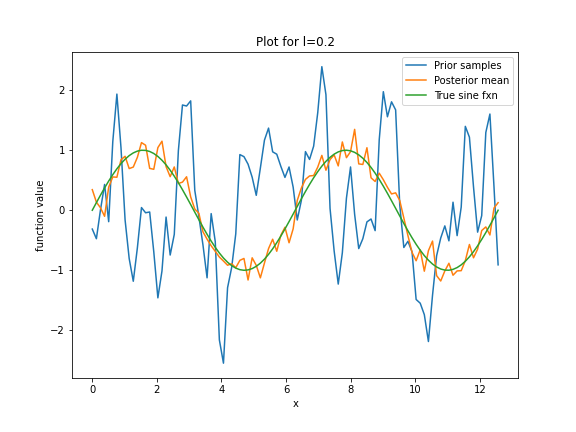
\includegraphics[height=2.65in]{question_4_0.2.png}
\caption{Plot for \(l=0.2\).} 
\label{fig:q4_02}
\end{figure}
\begin{figure}[h]
\centering
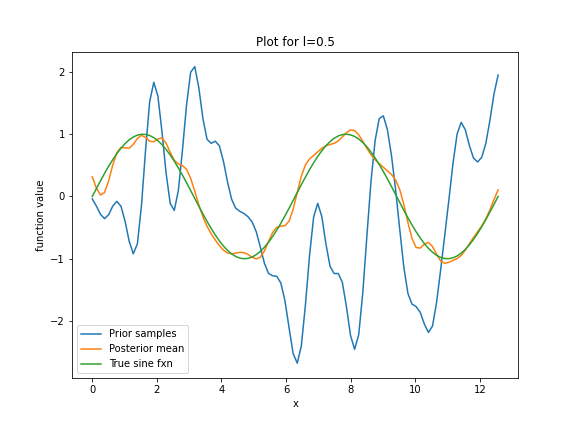
\includegraphics[height=2.65in]{question_4_0.5.png}
\caption{Plot for \(l=0.5\).} 
\label{fig:q4_05}
\end{figure}
\begin{figure}[h]
\centering
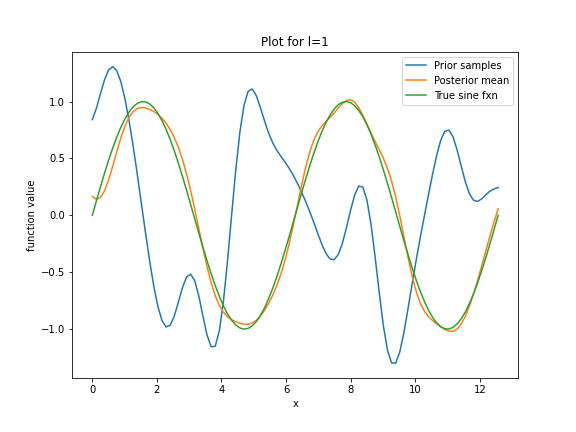
\includegraphics[height=2.65in]{question_4_1.png}
\caption{Plot for \(l=1.0\).} 
\label{fig:q4_1}
\end{figure}
\begin{figure}[h]
\centering
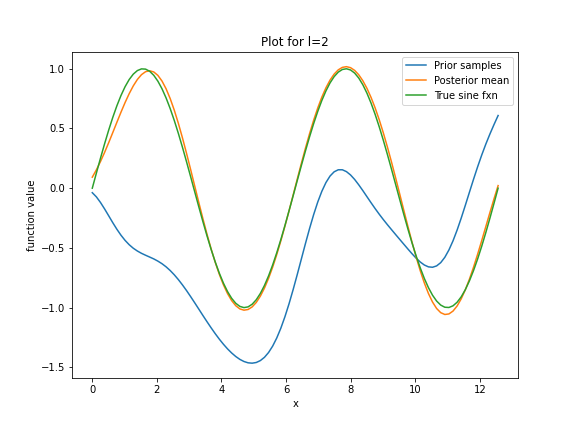
\includegraphics[height=2.65in]{question_4_2.png}
\caption{Plot for \(l=2.0\).}
\label{fig:q4_2}
\end{figure}
\begin{figure}[h]
\centering
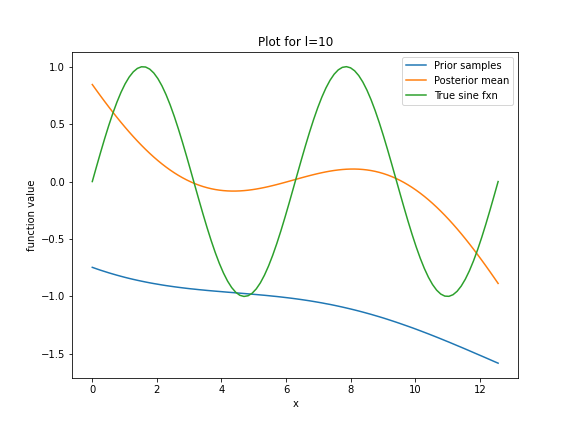
\includegraphics[height=2.65in]{question_4_10.png}
\caption{Plot for \(l=10\).} 
\label{fig:q4_10}
\end{figure}

\end{pmisolution}
\begin{pmisolution}
Given that the likelihood of each training output \(f_{n}\) has same form as GP regression's posterior predictive with \(\vZ,\vt\) as pseudo training data.\\
\[p(f_{n}|\vx_{n},\vZ,\vt) = \mathcal{N}(f_{n}| \tilde{\vk}_{n}\tilde{\vK}^{-1}\vt, \kappa(\vx_{n},\vx_{n})-\tilde{\vk}_{n}^{T}\tilde{\vK}^{-1}\tilde{\vk}_{n})\]
where \(\tilde{\vK}\) is \(M \times M\) kernel matrix, \(\tilde{\vk}_{n}\) is the \(M \times 1\) vector of kernel based similarities of \(\vx_{n}\) with pseudo inputs \(\vz_{1}, \vz_{2},.., \vz_{M}\).\\\\
\textbf{Posterior Predictive distribution}\\

Posterior predictive distribution for the output \(y_{\ast}\) of a new input \(\vx_{\ast}\)
\[ p(y_{\ast}|\vx_{\ast},\vX,\vf,\vZ) = \int p(y_{\ast}|\vx_{\ast},\vX,\vf,\vZ,\vt)p(\vt|\vX,\vf,\vZ)d\vt\]
and 
\[p(\vt|\vX,\vf,\vZ) = \frac{p(\vf|\vX,\vt,\vZ)p(\vt|\vZ)}{\int p(\vf|\vX,\vt,\vZ)p(\vt|\vZ)d\vt}\]
Now, calculating \(p(\vf|\vX,\vZ,\vt)\)
\[ p(\vf|\vX,\vZ,\vt) = \prod_{n=1}^{N}p(f_{n}|\vx_{n},\vZ,\vt) = \prod_{n=1}^{N}\mathcal{N}(f_{n}| \tilde{\vk}_{n}\tilde{\vK}^{-1}\vt, \kappa(\vx_{n},\vx_{n})-\tilde{\vk}_{n}^{T}\tilde{\vK}^{-1}\tilde{\vk}_{n}) = \mathcal{N}(\vf|\vR\Grave{\vK}^{-1}\vt,\vLambda)\]
where \(\vR_{nm} = \kappa(\vx_{n},\vz_{m})\), shape of \(\vR\) is \(N\times M\), \(\Grave{\vK}\) is \(M \times M\) matrix where each element \(\Grave{\vK}_{nm} = \kappa(\vz_{n},\vz_{m})\), \(\vLambda\) is \(N \times N\) diagonal matrix with diagonal element \(\vLambda_{nn} = \kappa(\vx_{n},\vx_{n}) - \vk_{n}^{T}\Grave{\vK}^{-1}\vk_{n}\).\\
\(p(\vt|\vZ)\) is gaussian with mean\(=0\) and co-variance matrix \(=\Grave{\vK}\). Using the conjugate property of gaussian for \(p(\vt|\vX,\vf,\vZ)\).\\
\[p(\vt|\vX,\vf,\vZ) = \mathcal{N}(\vt|\boldsymbol \mu_{t},\vSigma_{t})\]
where \( \boldsymbol \mu_t = \vSigma_{t}\Grave{\vK}^{-1}\vR^{T}\vLambda^{-1}\vf\) and \(\vSigma_{t} = \Grave{\vK}\vR^{-1}\vLambda{\vR^{T}}^{-1}\Grave{\vK}\).\\

Replacing \(y_{\ast} = f_{\ast}\), \(f(\vx_{\ast}) = \vk_{\ast}^{T}\Grave{\vK}^{-1}\vk_{\ast}\) and \(\epsilon \sim \mathcal{N}(0,\kappa(\vx_{\ast},\vx_{\ast}) - \vk_{\ast}^{T}\Grave{\vK}^{-1}\vk_{\ast})\) in GP regression formula where \(\vk_{\ast}\) is \(M \times 1\) vector with element \((\vk_{\ast})_{m} = \kappa(\vx_{\ast},\vz_{m})\). Therefore,
\begin{align*}
    p(f_{\ast}|\vx_{\ast}, \vX, \vf, \vZ) &= \mathcal{N}(f_{\ast}| \mu_{\ast}, \sigma_{\ast})\\
    &= \mathcal{N}(f_{\ast}| \vk_{\ast}^{T}\Grave{\vK}^{-1}\vSigma_{t}\Grave{\vK}^{-1}\vR^{T}\vLambda^{-1}\vf, \vk_{\ast}^{T}\Grave{\vK}^{-1}\vSigma_{t}\Grave{\vK}^{-1}\vk_{\ast} + \kappa(\vx_{\ast},\vx_{\ast}) - \vk_{\ast}^{T}\Grave{\vK}^{-1}\vk_{\ast})\\
\end{align*}
Now, this is evident that new computation cost is \(O(M^2N)\) due to the \(\vSigma_{t}\) computation in predictive posterior.\\\\
\textbf{Marginal Likelihood}\\
Given \(\vf = \vR\Grave{\vK}^{-1}\vt + \boldsymbol \epsilon\) where \(\boldsymbol \epsilon \sim \mathcal{N}(\boldsymbol 0,\vLambda)\) and linear Gaussian model.\\
\[p(\vf|\vX,\vZ) = \int p(\vf|\vX,\vZ,\vt)p(\vt|\vX,\vZ)d\vt = \mathcal{N}(\vf|\boldsymbol \mu_N,\vSigma_N)\]
where \(\boldsymbol \mu = \boldsymbol 0\) and \(\vSigma = \vR\Grave{\vK}^{-1}\vR^{T} + \vLambda\)\\
Using MLE-II for $\vZ$ computation and objective function,
\[\hat{\vZ} = \argmax_{\vZ}P(\vf|\vX,\vZ) = \argmax_{\vZ}\left[\frac{-1}{2}\log|\vSigma| - \frac{1}{2}\vf^{T}\vSigma^{-1}\vf\right] = \argmax_{\vZ}\left[\log|\vSigma| + \vf^{T}\vSigma^{-1}\vf \right]\]
\end{pmisolution}


\end{document}
